\documentclass[a4paper,titlepage,dvipdfmx]{jsarticle}

\usepackage{pxjahyper}
\renewcommand{\kanjifamilydefault}{\gtdefault} %For Japanese text

\usepackage[utf8]{inputenc} %Character code to utf-8
\usepackage{fancyhdr} % feader footer
\usepackage{lastpage}
\usepackage{graphicx}

\cfoot{\thepage}
\usepackage{listings} % sorcecode
\usepackage{inconsolata}

\renewcommand{\thelstnumber}{\arabic{lstnumber}:}
\lstset{language=C++,
  breaklines = true
  basicstyle = {10pt},
  basicstyle = \ttfamily,
  commentstyle = {\textit},
  keywordstyle = \bfseries,
  frame = tRBl,
}

\title{君はゲームプログラマーになりたいか? \\ 目指してるのは楽な道のりじゃないぜ}
\author{くらげ~}
\date{\today}

% From here text
\begin{document}
\maketitle

\section{君の名は?}
この上の君というの著作者だから心配する必要はない!

\subsection{ん?じゃあ君は宇宙人か?}
1IのJOKENの中で生きている(執筆時)くらげ~です。ん?人間なのにくらげ~とかみずみずしい名前しあがって、さてはてめえ宇宙人だな?
いや、別にただの一般人です。ま、プログラミングは8年、セキュリティは3年、人工知能は3ヵ月やってます。まあ、中身を詳しく言うときりがないので割愛しますが、何年やってきたかはどうでもいいんだよ!やる気さえあればなんでもできる!(白目)僕のモットーは広く深く、やり方は基礎を完全に理解してから、一気 に深く掘り下げていきます。それで勉強の効率化を図っています。僕の場合は基礎が定着 していないと応用をしないので、最初の方は成長が遅いです。小学校の時がそうやった。 

 僕は別にゲームクリエイターになるつもりは現時点ではないが、スキルを身に着ける上 で学習しながら OpenGL や Vulkan でオブジェクト配置したり GLSL(OpenGL Shading Language) で minecraft の影 mod(現時点では影処理しか書けない) を作ったりして楽し んでいる。ちなみに、影処理は Shadow mapping って調べたらでてくるぜ!その他にも いろいろしているが... まあ、そんなことはどうでもいい。ゲームプログラマーというものは知っているか?

\section{え?ゲームプログラマー?え、めっちゃかっこええやん}
この世には Unity や UNREAL ENGINE 4 など様々なゲームエンジンがあって、そ れで物理現象などを考えずにクリックで重力を起こせたり, さらにはオブジェクトを配置 したりできる。これらのゲームエンジンだけでゲームを作成することができる。ただ、君 はそこで満足するのか?ん?そこで満足していいと思ってるのか?

\subsection{基礎を知らないままゲームを作るのか?}
ゲームを作成するだけなら Unity や UNREAL ENGINE 4 の勉強をすればいい。で も、それはゲームクリエイターであってゲームプログラマーではない。ただ、これらの ゲームエンジンを使ってはいけないとは誰も言っていない。ゲームを作成するうえで時間 短縮、楽することは重要なことである。俺はゲームエンジンを使うことは推奨する人だ。 だが、どのように描画されているのか知らないままゲームエンジンでゲームを作成してい ると、ゲーム作成の基礎が分かっていないことになるよな?な?だから、ちょっとでも足 を突っ込んでみて、ゲームエンジンの中身までわからなくても、その初歩的なことでもわ かればそれでも十分だよな! (この資料に全部書くとページが何枚あっても足りないのは 秘密)

\section{本題に入る前に 2 次元/3 次元グラフィックスプログラミ ング API の紹介をするぜ}
まずは先ほど出てきたOpenGLからだ。こやつはクロノス・グループとかいうちょっとかっこいい名前をしているところが開発元だ。名前がかっこいいなみにやってることも侮れない。ちなみにこやつはCGAPI(コンピューターグラフィックスアプリケーションプログラミングインターフェイス)である。 

まあ、わけわからない言葉がたくさん出てきたが、不安がる必要はない。最初から分かる天才なんてこの世に存在しねえ。OpenGLってのはJava みたいに対応OSが幅広いのが特徴だ。ただ、C++みたいに簡単に学習できるような言語ではない少し複雑なAPIである。つい最近までは3Dゲームの作成などはこのAPIが主流であった(今も主流かも知 れない)。C++と併用するのが多い。 

次はDirectXというものだ。僕はこのAPIは少ししか触ったことがないので具体的にはいえないが。唯一いえることは、Windows のみでしか動作しないことだ。Windowsだけで動作させる場合ならこの選択肢もありだろう。 

その次にVulkanというものだ。こいつもクロノス・グループによって、開発されている。OpenGLの上位互換といってもいいAPIだ。ただOpenGLより難しいが、低レベルなAPIによって軽量な処理が可能になっている。今後主流になっていくであろうAPIであろう。 

その他にもいろいろあるかもしれないが、俺は知らない。

\section{おい、さっさと本題いってくれよ}
まあまあ、待て待て。今回紹介するのはOpenGLだが。同じ開発元だよな?じゃあ、何が違うんだ?

 A:同じ開発元だからなんだって言いたいんだ。
 
 me:いや... 別に何もないです....
 
\section{OpenGL と Vulkan の違いってなんだよ?}
何が違うかといわれても一見はほとんど違いはない。ただ簡単に言うとVulkanの方が多くのベンダーをサポートして効率的にGPUのリソースを使うことができる。何がVulkanの方が難しいか言うと、OpenGLではドライバによってメモリマネジメントや、スレッドマネジメント、コマンドバッファの生成や更新を自動でするが、Vulkanはそれをアプリケーション側でしないといけない。そこが難しい理由だ。ただ、勉強できないほど難しいものでもないので気になった人は勉強してみよう。そしてVulkanで描画したものはOpenGL内で使うことができるぞ!ただ、今回は紙媒体ということもあり、Vulkanのソースコードは長いので、資料に書くことができません!皆さんも読む気なくしますよね?

\newpage

\section{OpenGL}
まずはOpenGLで立方体を描画したいのだが、そもそもOpenGLってなんなの??

\subsection{OpenGLとは}
OpenGLとは,先ほど出たようにクロノス・グループ(khronos Group)が策定、開発していて、2/3次元CGAPIである。

\subsection{OpenGLとは何者だ!}
ここ最近、ゲームなどで3Dゲームなどが増えてきました。これは三次元コンピュータグラフィックス(3DComputerGraphics、3DCG)の技術を使っています。"Virtual Youtuber"などは3DCGなどを使って、キャラクターの外観を作成し、webカメラや今は生産終了されているKinectなどでモーションキャプチャーを行って、キャラクターを動かしたりしています。いま一番身近にある技術なのではないのかなと思っています。
ただ、"Virtual Youtuber"や3Dゲームが生まれる前からも、OpenGLは広く使われていました。一つの大きな要因としてOpenGLはプラットフォームに依存しないからです。プラットフォームに依存しないことによりLinuxのX Window Systemに組み込まれていたり、WindowsとmacOSともにOpenGLが導入されていて、さらにiOSやAndroidにも組込みシステム向けのOpenGL ESなどが導入されています。Nintendo SwitchもVulkanやOpenGLがサポートされています。

\subsection{OpenGLを動かすためには}
OpenGLは「プラットフォームに依存しないCGAPI(コンピュータグラフィックAPI)」であるが、やはりプラットフォームごとに少し工夫する必要があります。また、この工夫はちょっとめんどくさいのでそれを気にしなくて簡単に使うことができるキットがこの世には存在する。

\subsection{GLUT}
GLUTとは先ほどのキットの一種である。OpenGLの初期のころに作られたもので、僕も最初はこれを使って勉強していた。しかし、このGLUTには欠点があり、長期間メンテナンスされていないし、macOS ver10.9からはGLUTの使用が非推奨となっています。このキットはUnix系OSで使うことができるぞ!

\subsection{GLFW}
GLUTに代わるものしてQt(キュート)などたくさんありますが、やはり手軽に学習できるという点でGLFWをお勧めします。
GLFWはクロスプラットフォーム(マルチプラットフォーム)で、C言語で書かれているが、他の言語で使用することができるバインディングがある。
GLFWにはOpenGLのバージョンやプロファイルが指定できたりマルチモニタに対応していたり、いろいろ機能があるが説明しているときりがないので今回は省く。
さらに、このofflineではGLFWで描画するぜ!ちなみにゲームをOepnGLとC言語系で作るときはSDLの方が多機能でゲームプログラマー御用達なので、そっちを使うことをお勧めする。\newpage

\subsection{立方体を描画するぞ!}
OpenGLを使って図形を表示するソースコードを見たりプログラムを書いたりするにあたって、幾何学の存在は逃せません。とくに三次元空間のオブジェクトを扱うには、幾何学の知識が必要になります。

まずはソースコードを見てみよう!

\begin{lstlisting}[language=C++,numbers = left]
#define GLFW_INCLUDE_GLU
#include <iostream>
#include <GLFW/glfw3.h>
#define width 1280
#define height 960

static GLFWwindow*  window;

static const GLdouble CubeVertex[][3] = {
	{ 0.0, 0.0, 0.0 },
	{ 1.0, 0.0, 0.0 },
	{ 1.0, 1.0, 0.0 },
	{ 0.0, 1.0, 0.0 },
	{ 0.0, 0.0, 1.0 },
	{ 1.0, 0.0, 1.0 },
	{ 1.0, 1.0, 1.0 },
	{ 0.0, 1.0, 1.0 }
};

static const GLint CubeFace[][4] = {
	{ 0, 1, 2, 3 },
	{ 1, 5, 6, 2 },
	{ 5, 4, 7, 6 },
	{ 4, 0, 3, 7 },
	{ 4, 5, 1, 0 },
	{ 3, 2, 6, 7 }
};

static const GLdouble CubeNormal[][3] = {
	{ 0.0, 0.0,-1.0 },
	{ 1.0, 0.0, 0.0 },
	{ 0.0, 0.0, 1.0 },
	{ -1.0, 0.0, 0.0 },
	{ 0.0,-1.0, 0.0 },
	{ 0.0, 1.0, 0.0 }
};

static const GLfloat CubeMaterial[] = { 0.8f, 0.35f, 0.4f, 1.0f };
static const GLfloat Lightpos0[] = { 0.0f, 3.0f, 5.0f, 1.0f };


static void DrawCube()
{
	glMaterialfv(GL_FRONT_AND_BACK, GL_AMBIENT_AND_DIFFUSE, CubeMaterial);

	glBegin(GL_QUADS);
	for (size_t i = 0; i < 6; ++i)
	{
		glNormal3dv(CubeNormal[i]);
		for (size_t j = 0; j < 4; ++j)
		{
			glVertex3dv(CubeVertex[CubeFace[i][j]]);
		}
	}
	glEnd();
}

int main()
{

	if (glfwInit() == GL_FALSE)
	{
	std::cerr << "Error initilize GLFW" << std::endl;
	exit(EXIT_FAILURE);
	return 1;
	}
	
	glfwWindowHint(GLFW_CONTEXT_VERSION_MAJOR, 4);
	glfwWindowHint(GLFW_CONTEXT_VERSION_MINOR, 6);
	glfwWindowHint(GLFW_OPENGL_FORWARD_COMPAT, GL_TRUE);

	window = glfwCreateWindow(width, height, "SampleCube", NULL, NULL);

	if (window == NULL)
	{
		std::cerr << "Error create GLFW window." << std::endl;
		glfwTerminate();
		exit(EXIT_FAILURE);
		return 1;
	}

	glfwMakeContextCurrent(window);
	glEnable(GL_DEPTH_TEST);
	glEnable(GL_LIGHTING);
	glEnable(GL_LIGHT0);
	glEnable(GL_CULL_FACE);
	glCullFace(GL_FRONT);
	// #82ffe6 is HTML color
	glClearColor(0.509f, 1.0f, 0.901f, 1.0f);

	while (glfwWindowShouldClose(window) == GL_FALSE)
	{

		glClear(GL_COLOR_BUFFER_BIT | GL_DEPTH_BUFFER_BIT);
		glLoadIdentity();


		int now_width, now_height;
		glfwGetFramebufferSize(window, &now_width, &now_height);
		glViewport(0, 0, now_width, now_height);
		gluPerspective(30.0, (double)now_width / (double)now_height, 1.0, 100.0);
		glTranslated(0.0, 0.0, -2.0);
		gluLookAt(3.0, 5.0, 4.5, 0.0, 0.0, 0.0, 0.0, 1.0, 0.0);
		glLightfv(GL_LIGHT0, GL_POSITION, Lightpos0);

		DrawCube();

		glfwSwapBuffers(window);
		glfwPollEvents();
	}

	glfwTerminate();
	return 0;
}
\end{lstlisting}

この上記のコードはOpenGL(GLFW)における立方体の描画プログラムだ。早速見ていこう!

まず\verb|#|defineだ\verb|#|defineはC言語をベースとするプリプロセッサ命令で、マクロ処理を担っている。ちなみに\verb|#|define GLFW\verb|_|INCLUDE\verb|_|GLUはGLFW3.0以降にデフォルトでGLUヘッダーが含まれなくなったので、インクルードしています。
\verb|#|includeは\verb|#|defineと一緒でC言語をベースとするプリプロセッサ命令で。簡単に言うと別のソースファイルをまとめて処理してくれる。
\verb|#|include\verb|<|GLFW/glfw3.h\verb|>|が今回使うGLFWのソースファイルだ。これがないとGLFWを使うことができない。
\verb|#|define width 1280は横幅 \verb|#|define height 960は高さをマクロしている。ここでは初期のwindow sizeとして扱っている。

\subsection{ポリゴンの表示}

さあここから本場所に入っていく!C++ではint main(引数)※引数がvoidは省略可;がプログラム実行時に一番最初に呼び出される関数です。まず最初にすべきことはGLFWを初期化しないといけません。GLFWを初期化するのは以下のコードで初期化することができます

\begin{lstlisting}[language=C++]
if( !glfwInit() ) return 1;
\end{lstlisting}
僕のソースコードでは
\begin{lstlisting}[language=C++]
if (glfwInit() == GL_FALSE)
{
	std::cerr << "Error initilize GLFW" << std::endl;
	exit(EXIT_FAILURE);
	return 1;
}
\end{lstlisting}
このようになっていますが、あまり変わりはありません。!と== falseは同じ意味で、またfalseとGL\verb|_|FALSEも意味合い的にはそこまで違いはありません。また、
\begin{lstlisting}[language=C++]
std::cerr << "Error initilize GLFW" << std::endl;
\end{lstlisting}
と書いているのは、標準エラー出力を出した方がエラー内容が分かりやすいので、デバッグ時などに有用です。初期化に失敗した場合は
\begin{lstlisting}[language=bash]
Error initilize GLFW
\end{lstlisting}
と表示させ、初期化に失敗したとを知らせます。
\begin{lstlisting}[language=C++]
return 1;
\end{lstlisting}
で1を返して、プログラムが異常終了をします。\\
ちなみに余談なんですが
\newpage
\begin{lstlisting}[caption = sample.cpp,language = C++]
int main()
{
	return 0;
}
\end{lstlisting}
というソースコードがあって以下のコマンドを実行します\\Linux系のOSの場合は
\begin{lstlisting}[language=bash]
$ g++ sample.cpp
$ ./a.out && echo "SUCCESS"
\end{lstlisting}
Windowsの場合は
\begin{lstlisting}[language=bash]
$ g++ sample.cpp
$ ./a.exe && echo "SUCCESS"
\end{lstlisting}
そうすると出力はどうなるでしょうか?
では、次に下記のソースコードで同じコマンドを実行してみましょう。
\begin{lstlisting}[caption = sample.cpp,language = C++]
int main()
{
	return 1;
}
\end{lstlisting}
さて、どうなるでしょうか。一つ目のプログラムでコマンドを実行した場合、出力は
\begin{lstlisting}[language=bash]
SUCCESS
\end{lstlisting}
となりますが、2つ目プログラムでコマンドを実行した場合、出力はありません。
....で、何が言いたいの?まあ、returnの有用性を知ってもらいたかっただけです。
まあ、C++を普通に勉強するならいらない知識かもしれない。
\begin{lstlisting}[language=C++]
glfwWindowHint(GLFW_CONTEXT_VERSION_MAJOR, 4);
glfwWindowHint(GLFW_CONTEXT_VERSION_MINOR, 6);
glfwWindowHint(GLFW_OPENGL_FORWARD_COMPAT, GL_TRUE);
\end{lstlisting}
この3つは別に必要はないですが、window作成時に、コンテキストやスワップチェインなどの情報を指定します。
各環境によって動作するOpenGLのバージョンが変わってくる可能性があるので、
\begin{lstlisting}[language=C++]
glfwDefaultWindowHint();
\end{lstlisting}
を書くといいでしょう、これはデフォルトの情報を指定してくれます。
\begin{lstlisting}[language=C++]
window = glfwCreateWindow(width, height, "SampleCube", NULL, NULL);
\end{lstlisting}
ではwindowを作成する上で情報を指定します。
データ型としては
\begin{lstlisting}[language=C++]
glfwCreateWindow(int, int,const char, GLFWmonitor , GLFWwindow );
\end{lstlisting}
で構成されていて、第1引数は横幅、第2引数は高さ、第3引数は表示させるタイトル、第4引数は表示させるモニター、第5引数はリソースを共有するコンテキストです。また、GLFWwindow型のポインタを返します。ちなみにフルスクリーンにする方法があって、
\begin{lstlisting}[language=C++]
glfwCreateWindow(width, height, glfwGetPrimaryMonitor(), NULL );
\end{lstlisting}
glfwGetPrimaryMonitor()で1枚目のモニターを取得して、第4引数に渡しています。また、2枚目や3枚目のモニターをフルスクリーンにしたい場合は
\begin{lstlisting}[language=C++]
glfwCreateWindow(width, height, glfwGetMonitors(2), NULL );
\end{lstlisting}
で、フルスクリーンにさせることができます。
これもGLFWの初期化同様に、windowの生成に失敗したら1を返す必要があります。
僕のソースコードでは
\begin{lstlisting}[language=C++]
if (window == NULL)
{
	std::cerr << "Error create GLFW window." << std::endl;
	glfwTerminate();
	exit(EXIT_FAILURE);
	return 1;
}
\end{lstlisting}
となっていますが
\begin{lstlisting}[language=C++]
if (!window)
{
	glfwTerminate();
	return 1;
}
\end{lstlisting}
でOKです。なぜglfwTerminate();が必要なのかというと、glfwInit関数を呼び出した後は必ず呼び出す必要があるからです。
そして、glfwMakeContextCurrentを使ってカレントにします。
\begin{lstlisting}[language=C++]
glfwMakeContextCurrent(window);
\end{lstlisting}
OpenGLのAPIを使う前には、必ずOpenGLコンテキストを取得しなければならないのでこのコードは必須です。
他のコンテキストをカレントするか、もしくはウィンドウが破棄(主に終了動作)されるまで、カレントコンテキストはこの状態を維持し続けます。\\
OpenGLのAPIを使えるようになったので、まずはOpenGLを初期化していきます。
まずはデプスバッファの有効化です。
\begin{lstlisting}[language=C++]
glEnable(GL_DEPTH_TEST);
\end{lstlisting}
で有効化できるのですが....デプスバッファって何?

デプスバッファとはZバッファとも呼ばれますが、深度情報を用いて物体の描画処理を省略して高速化するための技術です。
3DCGでは、平面に描画するためには空間内に配置された物体の頂点や境界線、表面のうち見えている部分だけを描画しなければなりません。手前にある他の物体などに隠されて見えてない部分の描画を省略する必要があるから有効にしています。今回は1つの物体しか描画していませんが、2つ3つ描画するときに必要なものです。

その次に、ライティング処理を有効化します。
\begin{lstlisting}[language=C++]
glEnable(GL_LIGHTING);
\end{lstlisting}
これで頂点カラーに証明パラメーターを使用するようになりました。そして光源を有効化します。
\begin{lstlisting}[language=C++]
glEnable(GL_LIGHT0);
\end{lstlisting}
でライト0が有効化されました。
\begin{lstlisting}[language=C++]
glEnable(GL_CULL_FACE)
\end{lstlisting}
描画処理を軽量化します。これではポリゴンの片面表示を有効化しています\\
表面だけ描きたいのなら
\begin{lstlisting}[language=C++]
glCullFace(GL_BACK);
\end{lstlisting}
裏面だけを描きたいのなら
\begin{lstlisting}[language=C++]
glCullFace(GL_FRONT);
\end{lstlisting}
両面を描くときは、
\begin{lstlisting}[language=C++]
glDisable(GL_CULL_FACE);
\end{lstlisting}
を一応書いた方がいいでしょう。
そして、glClearColor()でglViewPortで指定した範囲を塗りつぶします。
ちなみにglClearColorはRGBAで指定できるのですが、少し気を付けなければならない点があります。
256段階の数字を扱うのではなく係数で扱います。すなわち、1.0が255で0.0が0となります。なので\verb|#|82ffe6はrbga(130,255,230,1.0)になって係数にするには、$ y = \frac{x}{255} $に当てはめて計算します。すると
\begin{lstlisting}[language=C++]
glClearColor(0.509f, 1.0f, 0.901f, 1.0f);
\end{lstlisting}
こう書けます!!
GLFWでは描画する際にwhileでループを書かなければなりません。
\begin{lstlisting}[language=C++]
while(!glfwWindowShouldClose())
\end{lstlisting}
でできます。
glClear()を用いれば、バッファを初期化できます。
\begin{lstlisting}[language=C++]
glClear(GL_COLOR_BUFFER_BIT | GL_DEPTH_BUFFER_BIT);
\end{lstlisting}
GL\verb|_|COLOR\verb|_|BUFFER\verb|_|BITは色バッファの初期化、GL\verb|_|DEPTH\verb|_|BUFFER\verb|_|BITはデプスバッファ(Zバッファ)を初期化します。
\begin{lstlisting}[language=C++]
glLoadIdentity();
\end{lstlisting}
をコールして変換行列を単位行列で初期化します。これで描画毎に座標系をリセットしています。
\begin{lstlisting}[language=C++]
int now_width, now_height;
glfwGetFramebufferSize(window, &now_width, &now_height);
\end{lstlisting}
now\verb|_|widthとnow\verb|_|heightのint型を宣言して、glfwGetFramebufferSize()でフレームバッファサイズを取得します。そして、
\begin{lstlisting}[language=C++]
glViewport(0, 0, now_width, now_height);
\end{lstlisting}
でglClearColorで設定された色をglViewportの範囲を塗りつぶします。
\begin{lstlisting}[language=C++]
gluPerspective(30.0, (double)now_width / (double)now_height, 1.0, 100.0);
\end{lstlisting}
gluPerspective()では視野角、奥行きの最大、最小距離を描画します。この範囲外は例外を除いて基本的には描画されません。
第1引数には縦の視野角(度数指定)、第2引数には縦に対する横方向の視野角、第3引数には一番近いZ座標を指定して、第4引数には一番遠いZ座標を指定します
\begin{lstlisting}[language=C++]
glTranslated(0.0, 0.0, -2.0);
\end{lstlisting}
glTranslated()ではx,y,zに移動量を渡すと、平行移動します。
この場合z軸方向に-2.0平行移動します。
そして、カメラの位置と姿勢を設定します
\begin{lstlisting}[language=C++]
gluLookAt(3.0, 5.0, 4.5, 0.0, 0.0, 0.0, 0.0, 1.0, 0.0);
\end{lstlisting}
左に引数から順にカメラのX座標,Y座標,Z座標,注視点のX座標,注視点のY座標,注視点のZ座標、カメラの上方向がX軸に対してどこか,カメラの上方向がY軸に対してどこか,カメラの上方向がZ軸に対してどこかを指定します。第7,8,9引数はベクトルを指定します。
\begin{lstlisting}[language=C++]
glLightfv(GL_LIGHT0, GL_POSITION, Lightpos0);
\end{lstlisting}
第2引数でGL\verb|_|POSITIONが定数とされているので、光源を設置します。Lightpos0の座標に設置します、その後にDrawCube()を呼び出します。

\subsection{DrawCube()}
まずはオブジェクトの質を設定します
\begin{lstlisting}[language=C++]
glMaterialfv(GL_FRONT_AND_BACK, GL_AMBIENT_AND_DIFFUSE, CubeMaterial);
\end{lstlisting}
第1引数には質感を適用する面を指定します。GL\verb|_|FRONT\verb|_|AND\verb|_|BACKは両面を指定しています。そして第2引数では反射光を指定します、GL\verb|_|AMBIENT\verb|_|AND\verb|_|DIFFUSEになっているので、拡散反射係数と鏡面反射係数の両方を保持しています。
次に描く処理を書きます。glBegin()から始まってglEnd()の間を処理します。
その次にglNormal3dv()で法線ベクトルの設定を行います。オブジェクトが都のように光が反射するかどうかはこれによって決まります。
最後にglVertex3dv()で配列のポインタを与えて頂点を指定します。
forとかでソースコードの解読が困難になっていますが、可視化すると
\begin{lstlisting}[language=bash]
CubeNormal: { 0.0 ,0.0 ,-1.0 }

-----------------------------
CubeVertex: { 0.0 ,0.0 ,0.0 }
CubeVertex: { 1.0 ,0.0 ,0.0 }
CubeVertex: { 1.0 ,1.0 ,0.0 }
CubeVertex: { 0.0 ,1.0 ,0.0 }
-----------------------------

CubeNormal: { 1.0 ,0.0 ,0.0 }

-----------------------------
CubeVertex: { 1.0 ,0.0 ,0.0 }
CubeVertex: { 1.0 ,0.0 ,1.0 }
CubeVertex: { 1.0 ,1.0 ,1.0 }
CubeVertex: { 1.0 ,1.0 ,0.0 }
-----------------------------

CubeNormal: { 0.0 ,0.0 ,1.0 }

-----------------------------
CubeVertex: { 1.0 ,0.0 ,1.0 }
CubeVertex: { 0.0 ,0.0 ,1.0 }
CubeVertex: { 0.0 ,1.0 ,1.0 }
CubeVertex: { 1.0 ,1.0 ,1.0 }
-----------------------------

CubeNormal: { -1.0 ,0.0 ,0.0 }

-----------------------------
CubeVertex: { 0.0 ,0.0 ,1.0 }
CubeVertex: { 0.0 ,0.0 ,0.0 }
CubeVertex: { 0.0 ,1.0 ,0.0 }
CubeVertex: { 0.0 ,1.0 ,1.0 }
-----------------------------

CubeNormal: { 0.0 ,-1.0 ,0.0 }

-----------------------------
CubeVertex: { 0.0 ,0.0 ,1.0 }
CubeVertex: { 1.0 ,0.0 ,1.0 }
CubeVertex: { 1.0 ,0.0 ,0.0 }
CubeVertex: { 0.0 ,0.0 ,0.0 }
-----------------------------

CubeNormal: { 0.0 ,1.0 ,0.0 }

-----------------------------
CubeVertex: { 0.0 ,1.0 ,0.0 }
CubeVertex: { 1.0 ,1.0 ,0.0 }
CubeVertex: { 1.0 ,1.0 ,1.0 }
CubeVertex: { 0.0 ,1.0 ,1.0 }
-----------------------------

\end{lstlisting}
glNormal3dv()にはCubeNormal:の後の配列を、glVertex3dv()にはCubeVertex:の後の配列を与えて頂点を指定しています。

\begin{lstlisting}[language=C++]
glfwSwapBuffers(window);
glfwPollEvents();
\end{lstlisting}
そしてglfwSwapBuffers()とglfwPollEvents()で描画用バッファをスワップします。

\subsection{GLFWの終了}
glfwWindowShouldClose(window)がTRUEになるとループが終わるため、GLFWの終了処理が必要です。
\begin{lstlisting}[language=C++]
glfwTerminate();
return 0;
\end{lstlisting}
glfwTerminateはプログラムの最後に呼び出さないといけないおまじないです。そしてreturn 0;でプログラムが正常終了したことを伝えます。ちなみに今回作った図形はこちらです


\begin{center}
 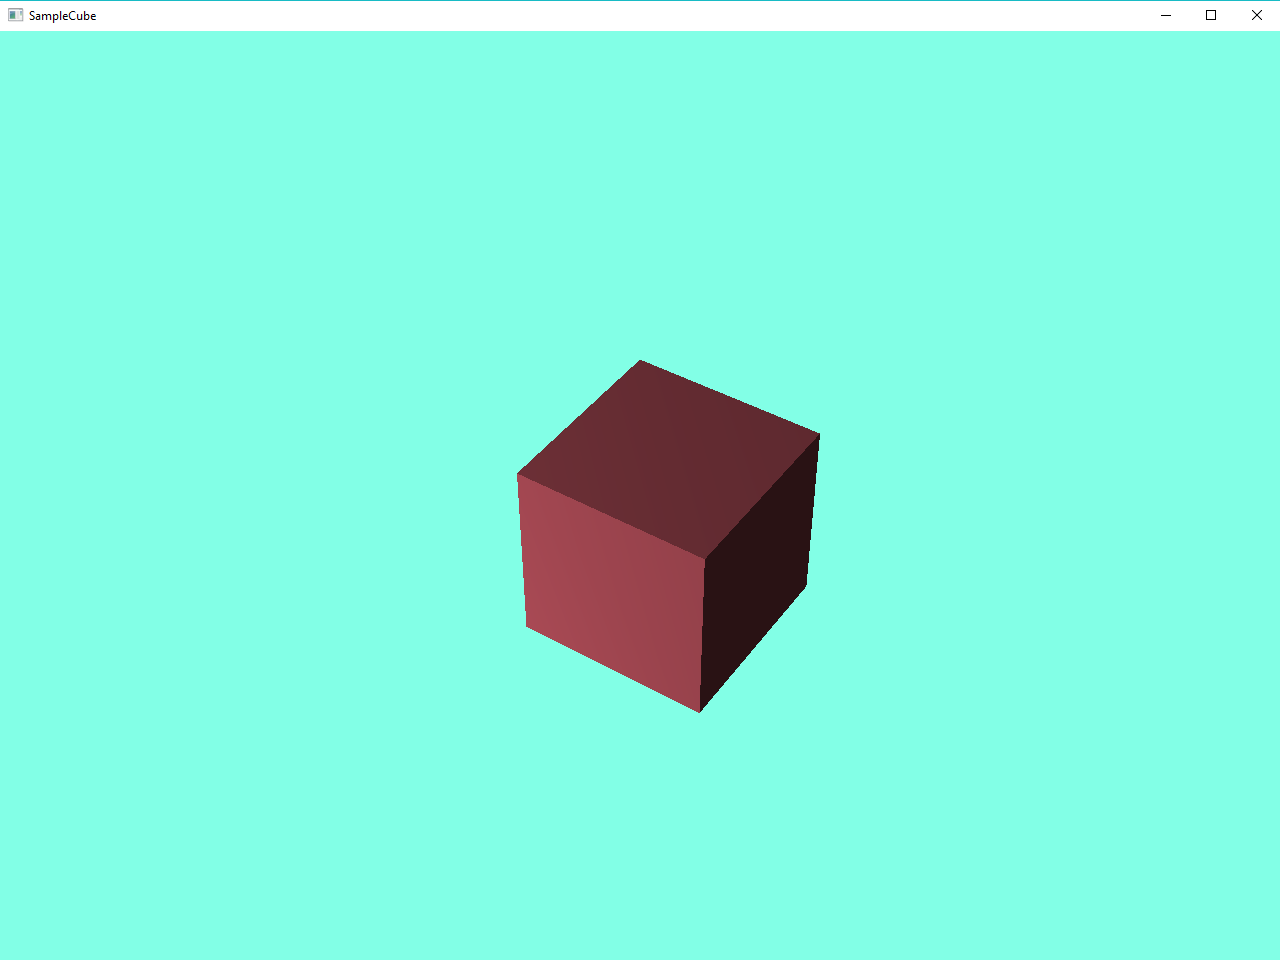
\includegraphics[width=8cm]{SampleCube.png}
\end{center}

\section{さいごに}
今回はofflineでVulkanとかOpenGLで立方体を回転させてみたり、変形させてみたりはしていませんが。OpenGLやvulkanではそんなこともできます。僕は楽しいからプログラミングをやっています。プログラミングはたのしいですよ?!jokenではプログラミングを学ぶことができたりします!
(最初のような感じで書こうと思ったが...案外難しかった)

\begin{thebibliography}{99}
\bibitem{b_0} ''GLFW Documentation'' \\
 http://www.glfw.org/documentation.html \\
 http://www.glfw.org/docs/latest/index.html \\
 http://www.glfw.org/docs/latest/pages.html \\
 http://www.glfw.org/docs/latest/modules.html
\bibitem{b_1} ''OpenGL 4.6 API Reference Guide'' \\
 https://www.khronos.org/files/opengl46-quick-reference-card.pdf
\bibitem{b_2} ''GLUTによる「手抜き」OpenGL入門'' \\
 ・座標データの参考にしました。\\
 https://tokoik.github.io/opengl/libglut.html\verb|#|8
\end{thebibliography}


\end{document}

